\documentclass[11pt,letterpaper]{article}
\usepackage{array}
\usepackage[in]{fullpage}
\usepackage{verbatim}
\usepackage{parskip}
\usepackage{graphicx}
\usepackage{rotating}

\usepackage{titlesec}
\titlespacing{\section}{0pt}{\baselineskip}{0pt}
\titleformat*{\section}{\normalsize\bfseries\MakeUppercase}

\titlespacing{\subsection}{0pt}{0.5\baselineskip}{0pt}
\titleformat*{\subsection}{\normalsize\bfseries}

\titlespacing{\subsubsection}{0pt}{0.5\baselineskip}{0pt}
\titleformat*{\subsubsection}{\normalsize\itshape}

%\setlength{\parindent}{0in}

\begin{document}
\setlength{\parindent}{0in}
%\baselineskip 4pt
\newcommand{\tablespace}[0]{\vspace{8pt}}
\textbf{ENVS S422: Earth's Climate System\\
Modeling Exercise 7: The carbon cycle}\\%\footnote{Based on exercises developed by Dave Bice at Penn State University.}}\\

In this exercise you will be modeling the short-term carbon cycle to investigate how various forcings, including carbon emissions and land use changes, can modify atmospheric CO$_2$ and other carbon reservoirs over timescales of years to a few centuries. The model that I'm providing you with is set-up to be in a steady state and consistent with conditions in the late 1880's. By adding known CO$_2$ emissions since the industrial revolution, we can test how well the model captures observed changes in CO$_2$ concentrations. Once we have confidence in the model, we can begin to test how the model responds to things like volcanic eruptions and we can model changes in the carbon cycle due to future CO$_2$ emissions.

For each model experiment, you should submit a brief 1-paragraph response to the questions that are being explored in the exercise and \textit{at least} one graph to help justify your response.

Due date: 15 April 2019


\section{Model description}
The global carbon cycle model that you will be using (Fig. \ref{fig:gcc})  consists of the short-term terrestrial and marine organic carbon cycles as well as steady fluxes from the inorganic carbon cycle. The model includes six reservoirs: fossil fuels, the atmosphere, land biota, soil, the surface ocean, and the deep ocean. The initial volumes of the reservoirs are based on estimates from the IPCC (Intergovernmental Panel on Climate Change) reports. These reservoirs are connected by several flows, which I discussed in lecture and will summarize below.

\begin{sidewaysfigure}
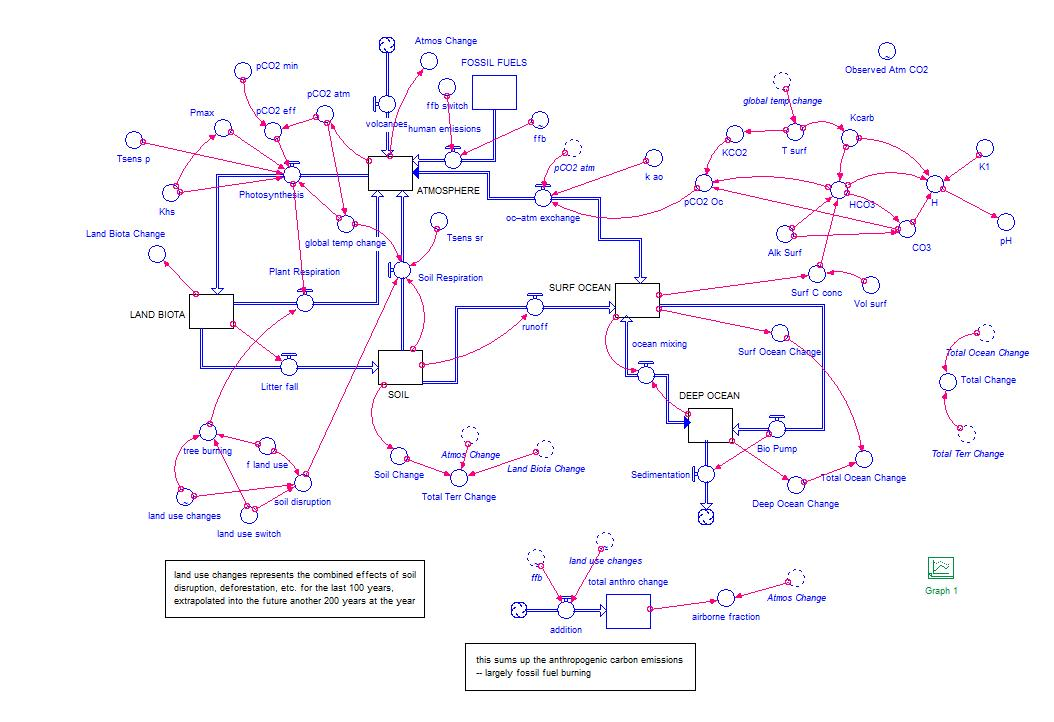
\includegraphics[width=\textheight]{./global_carbon_cycle_model.jpg}
\caption{Stella model of the (short-term) global carbon cycle.}
\label{fig:gcc}
\end{sidewaysfigure}

	
\subsection*{Flows}
\subsubsection*{Photosynthesis and respiration}
Carbon is exchanged between the atmosphere and the terrestrial biota through photosynthesis and respiration. In photosynthesis, plants convert CO$_2$ and H$_2$O into carbohydrates and O$_2$. Photosynthetic rates depend on CO$_2$ concentrations and air temperature. At low levels of CO$_2$, an increase in CO$_2$ results in increased photosynthetic rates. There is an upper limit to this effect, such that changes in CO$_2$ concentrations have little effect on photosynthesis when CO$_2$ concentrations are already high. The dependency of photosynthesis on temperature is similar, in that increases in temperature tend to increase photosynthetic rates so long as the temperature isn't high enough to destroy important enzymes. (We are unlikely to reach temperatures that high over the next few centuries, and so we can safely ignore that effect in our simulations.) High air temperatures are also thought to lead to more precipitation, which can also increase productivity because plant growth is often limited by water supply. Thus, we need to keep track of temperature, which we will do by setting
%\begin{equation}
%\Delta T = (p\mbox{CO}_{2,atm}-280)*0.01^\circ\mbox{C},
%\end{equation}
\begin{equation}
\Delta T = 2.5\frac{\ln(p\mbox{CO}_{2,atm}/290)}{\ln 2}
\end{equation}
where $\Delta T$ is the change in temperature relative to the pre-industrial temperature of 14$^\circ$C, $p\mbox{CO}_{2,atm}$ is the concentration of CO$_2$ in the atmosphere, and 290 ppm (parts per million is the initial concentration of CO$_2$. This equation results in an increase in air temperature of 2.5$^\circ$C for each doubling of CO$_2$.

To model photosynthesis on a global scale, we need to come up with a formula that is consistent with the following observations of photosynthesis:
\begin{itemize}
\item the global flow should be about 100 Gt C/yr;
\item the rate should increase with CO$_2$ levels, but there should be a saturation point, beyond which increases in atmospheric CO$_2$ yields no further increase in the rate of photosynthesis; and
\item the rate should increase with increasing temperature.
\end{itemize}
There are several ways this could be done; we will use the following formulation:
\begin{equation}
F_p = \left(\frac{P_{max}\times p\mbox{CO}_{2,eff}}{K_{hs}+p\mbox{CO}_{2,eff}}\right)\left(1+T_{sens,p}\Delta T\right),
\end{equation}
where $F_p$ is the global rate of photosynthetic uptake (or gross primary productivity), $P_{max}$ is a parameter that is used to force the equation for $F_p$ to give the proper value for the starting conditions of the model (kind of like a y-intercept), $p\mbox{CO}_{2,eff}=p\mbox{CO}_{2}-p\mbox{CO}_{2,min}$ is the effective CO$_2$ concentration, $p\mbox{CO}_{2,min}=30$~ppm is the minimum CO$_2$ concentration for photosynthesis, and $T_{sens,p}=0.07$ is the sensitivity of the photosynthetic uptake per degree of warming. $P_{max}$ is defined as
\begin{equation}
P_{max} = \frac{(K_{hs}+(p\mbox{CO}_{2,i}-p\mbox{CO}_{2,min}))*F_{p,i}}{p\mbox{CO}_{2,i}-p\mbox{CO}_{2,min}},
\end{equation}
where $K_{hs}=72.5$~ppm is the half saturation value (i.e., the CO$_2$ concentration at which rate of photosynthesis is half of the maximum value), $p\mbox{CO}_{2,i}=290$~ppm is the initial (pre-industrial) CO$_2$ concentration, and $F_{p,i}=100$~Gt C/yr is the initial photosynthetic uptake. Note that $K_{hs}$ is a key parameter affecting the shape of the $F_p$ curve, and that the curve varies linearly with temperature (if CO$_2$ is held fixed).

We will use a much simpler formulation for respiration, which is based on experiments that indicate that the ratio of photosynthesis to respiration is commonly around 2. Thus, we will set
\begin{equation}
F_{pr}=0.5*F_p+\mbox{tree burning},
\end{equation}
where $F_{pr}$ is the rate of global plant respiration. See section on \textbf{Human impacts} for discussion of tree burning.

\subsubsection*{Litter fall}
Dead plant material enters the soil in two ways --- it falls on the surface as litter, and it is contributed below the surface from roots. The relative importance of these two pathways into the soil carbon reservoir vary according to the plants in an ecosystem, but it appears that the two are commonly about equal. In our model, we will lump these processes together and call them litter fall, keeping in mind that this is only half of the real story. Litter fall is set to be the difference between the photosynthetic uptake of carbon and the return of carbon through plant respiration. If this were not the case, then the size of the land biota reservoir would be growing or declining, which may in fact be the case (it's doing both in different parts of the Earth), but we would like our model to be more or less in a steady state initially. In reality, it is the litter fall that is actually measured in studies of carbon flow through ecosystems; that, combined with a measure of the gross primary productivity (the total amount of carbon used in photosynthesis) gives an estimate of the plant respiration flow according to the following equation:
$$\mbox{Gross Primary Productivity = Plant Respiration + Litter Fall}$$
Having already chosen the initial rates for photosynthesis and plant respiration, at 100 and 50, this leaves us with a value of 50 Gt C/yr for the rate of carbon added to the soil reservoir through the process of litter fall. But, we don't want this to be a constant value; it will undoubtedly change as a function of the size of the land biota reservoir. So, we can define this flow in the form of a standard draining flow,
\begin{equation}
F_{lf} = 50\left(\frac{\mbox{land\_biota}}{\mbox{INIT(land\_biota)}}\right) 
\end{equation}
where $F_{lf}$ is the flow in Gt C/yr and $\mbox{land\_biota}$ is the amount of carbon stored in the land biota (plants) at any given time.

\subsubsection*{Soil respiration}
Respiration also occurs within the soil, as microorganisms consume the dead plant material. In terms of a chemical formula, this process is the same as described above for plant respiration (at least for aerobic decomposition), only in this case, the microbes do not make the fuel themselves.

Much of the organic material added to the litter (the accumulated material at the surface of the soil) or within the root zone each year is almost completely consumed by microbes; thus there is a reservoir of carbon with a very fast turnover time --- on the order of 1 to 3 years in many cases. The by-products of this microbial consumption are CO$_2$, H$_2$O, and a
variety of other compounds, collectively known as humus. Humus is much less palatable compound, as far as microbes are concerned, and is not decomposed very quickly. After it is produced at shallow levels within soil, it generally moves downward and accumulates in regions of the soil with high clay content. Part of the reason it accumulates in the lower parts of the soil is that there tends to be less oxygen in that environment, and the lack of oxygen makes it even more difficult for microbes to work on this humus and decompose it further. But eventually, due to various processes that stir the soil, this humus moves back up to where there is more oxygen and then the microbes will eventually destroy the humus and release some more CO$_2$. This humus then constitutes another, longer-lived reservoir of carbon in the soil that has a residence time of \~25 years.

Decomposition rates are very sensitive to the organic carbon content of the soil as well as the temperature and water content, respiring faster at higher carbon concentrations, higher temperatures and in moister conditions (unless the soil is flooded). Soil respiration is likely even more sensitive to temperature than photosynthesis and plant respiration. In general, higher temperatures tend to correspond with higher rates of precipitation, so we can consider the effects of water to go hand in hand with temperature. In our model of the carbon cycle, we will use an expression for the rate of soil respiration, $F_{sr}$ that depends linearly on temperature and is proportional to the amount of carbon stored in soil:
\begin{equation}
F_{sr} = 49.4\left(\frac{\mbox{Soil}}{\mbox{INIT(Soil)}}\right)*(1+T_{sens,sr}\Delta{T})+\mbox{soil disruption},
\end{equation}
where $T_{sens,sr}=0.1$ is the sensitivity of soil respiration per degree of warming. The formulation here gives an increase in soil respiration by a factor of 2.0 if the temperature increases 10$^\circ$C. It is important to note once again that there is an upper limit to this temperature sensitivity function in the real world, but we do not expect to approach it in this modeling exercise and therefore do not incorporate it into our equation. See section on \textbf{Human impacts} for discussion of soil disruption.

\subsubsection*{Runoff}
Although most of the carbon loss from the soil reservoir occurs through respiration, some carbon is transported away by water running off over the soil surface. This runoff is eventually transported to the (surface) oceans by rivers. The actual magnitude of this flow is a bit uncertain, although it does appear to be quite small. The most recent estimates place it at 0.6 Gt C/yr. We will define the runoff, $F_{ro}$ using a standard draining flow:
\begin{equation}
F_{ro} = 0.6\left(\frac{\mbox{soil}}{\mbox{INIT(soil)}}\right).
\end{equation}

\subsubsection*{Ocean-atmosphere exchange}
In the inorganic carbon cycle, carbon is continuously exchanged between the surface ocean and the atmosphere. The rate and direction (note that this flow is a bi-flow) depend on the difference in concentrations between the ocean and the atmosphere. We will model the exchange using
\begin{equation}
F_{oc-atm} = k_{ao}\left(p\mbox{CO}_{2,atm}-p\mbox{CO}_{2,oc}\right),
\end{equation}
where $k_{ao}=0.278$ (Gt C)/(yr$\cdot$ppm) is an empirically determined coefficient. The concentration of CO$_2$ in the surface ocean, $p\mbox{CO}_{2,oc}$, through a series of equations that describe carbonate chemistry (see web of converters and connectors in Fig. \ref{fig:gcc}). I won't go into details here, but note that they are derived from the equations that we used to describe how CO$_2$ can react with water to form carbonic acid, bicarbonate ions, and carbonate ions.

\subsubsection*{Ocean mixing}
The ocean mixing flow, which is a bi-flow, accounts for upwelling and downwelling that occurs as a result of thermohaline circulation.

As we discussed earlier in the semester, downwelling transfers cold surface waters into the deep interior of the oceans, and as a result, carbon is transferred as well. The magnitude of the flow is thus a function of the water flux and the average concentration of carbon in the surface waters, which is itself a function of the total amount of carbon stored in this reservoir (assuming that the size of the reservoir is not changing appreciably during the simulations). Upwelling is the converse of downwelling, and as the deep waters rise to the surface, they bring with them carbon. The total transfer of carbon is thus a function of the volume of water involved in this flow and the amount of carbon stored in the deep ocean reservoir. Upwelling occurs in areas of the oceans where winds and surface currents diverge, moving the surface waters away from a region; in response, deep waters rise up to fill the "void". Upwelling occurs along the equator, where there is a strong divergence, and also along the margins of some continents, such as the west coast of South America. This upwelling water also brings with it nutrients such as nitrogen and phosphorus, making these waters highly productive.

We will define this bi-flow according to
\begin{equation}
F_{om} = 100\frac{\mbox{deep\_ocean}}{\mbox{INIT(deep\_ocean)}}-90.6\frac{\mbox{surf\_ocean}}{\mbox{INIT(surf\_ocean)}}.
\end{equation}
In the initial, steady-state solution for the model, there will be 100 Gt C/yr being upwelled and 90.6 Gt C/yr being downwelled. These values are consistent with observations but have been adjust to create a steady-state model.

Note that the amount of carbon transferred by this upwelling is greater than the amount transferred by downwelling, so that this flow is (at least initially) positive. This is not because the volume of flow is different in these two processes, but rather because the concentration of carbon in the deep waters of the ocean is greater than that in the shallow surface waters, due in part to the operation of the biologic pump described below.

\subsubsection*{Biological pump}
Phytoplankton, which reside in surface waters, utilize CO$_2$ in seawater to create organic matter. Just like terrestrial plants, when these phytoplankton die they respire, transfer CO$_2$ back to the water. At the same time, many planktonic organisms extract dissolved carbonate ions from seawater and turn them into CaCO$_3$ shells. These organisms generally decompose very quickly when they die, but some of the organic matter and the inorganic shells sink to the deep water, thus removing carbon from the surface waters.  

The rate at which carbon is removed from the surface waters and pumped into the deep water depends on marine productivity, which is itself a complex function of water temperature, nutrient availability, etc. Since we are not modeling those things we are forced to adopt a much simpler approach --- we will simply assume a constant flow rate of $F_{bm}=10$~Gt~C/yr.


\subsubsection*{Sedimentation}
Some of the carbon, both organic and inorganic (i.e., calcium carbonate shells) produced by marine biota and transferred to the deep oceans settles out onto the sea floor and accumulates there, eventually forming sedimentary rocks. The magnitude of this flow is small, about 0.6 Gt C/yr, relative to the total amount transferred by sinking from the surface waters. The reason for this difference is primarily because the deep waters of the oceans dissolve calcium carbonate shell materials; below about 4 km, the water is so corrosive that virtually no calcium carbonate material can accumulate on the sea floor. In addition, some of the organic carbon is consumed by organisms living in the deep waters and within the sedimentary material lining the sea floor. This consumption results in the release of CO$_2$ into the bottom waters and thus decreases the amount of carbon that is removed from the ocean through this process. It is worth noting that the process of organic carbon consumption on the seafloor is another microbial process and is very similar to the soil respiration flow described above. Since the microbes living on the seafloor require oxygen to accomplish this task, the supply of oxygen to the seafloor by deep currents is an important part of this process.

We will simply define the sedimentation flow to be a fixed percentage of the amount of carbon transferred to the deep waters by the biologic pump flows from the shallow marine biota reservoirs. The equation for this flow is thus:
\begin{equation}
F_{sed} = 0.06\times F_{bm}
\end{equation}

where Fsed is the transfer of carbon from the deep ocean reservoir to the sedimentary rock reservoir, and Fswob and Fscob are the flows of carbon from the warm and cold surface ocean biota. This equation is set up so that initially, with Fswob and Fscob set to total 10 Gt C/yr, the Fsed flow will have a value of 0.6 Gt C/yr.

\subsubsection*{Volcanism and metamorphism}
When sedimentary rocks deposited on oceanic crust are subducted, they may melt or undergo metamorphism; in either case, the carbon stored in calcium carbonate (i.e., limestone) is liberated in the form of CO$_2$, which is ultimately released at the surface. The CO$_2$ may come out when a volcano erupts or it may slowly diffuse out from the interior via hot springs, but in both cases it represents a transfer of carbon from the reservoir of sedimentary rocks to the atmosphere. 

The magnitude of this flow is quite small, and is adjusted here to a value of 0.6 Gt C/yr in order to create a model in steady state. This flow is defined as a constant in the model, although in reality, it will vary according to the timing of large volcanic eruptions. An extremely large volcanic eruption may emit carbon at a rate of around 0.2 Gt C/yr for a year or two, creating a minor fluctuation.

\subsection*{Human impacts}
\subsubsection*{Human emissions}
Humans are directly emitting carbon, especially CO$_2$, directly into the atmosphere. Since we know the rates at which we are consuming fossil fuels, we have very good estimates of our CO$_2$ emissions. Current rates are about 6 Gt C/yr. In the simulations you will modify CO$_2$ emission rates to explore how our emissions affect the global carbon cycle.

\subsubsection*{Land use changes}
The other form of human alteration of the global carbon cycle is through forest cutting and burning and the disruption of soils. When deforestation occurs, most of the plant matter is either left to decompose on the ground or it is burned, the latter being the more common occurrence. This process reduces the size (the mass) of the land biota reservoir and the burning adds carbon to the atmosphere. Land-use changes other than deforestation can also add carbon to the atmosphere; agriculture, for instance, involves tilling the soil, which leads to very rapid decomposition and oxidation of soil organic matter. This means that in terms of a system, we are talking about two separate flows here --- one draining the land biota reservoir, the other draining the soil reservoir; both flows transfer carbon to the atmosphere. Current estimates place the total addition to the atmosphere from forest burning and soil disruption at around 1.5 Gt C/yr; estimates divide this into 70\% to 50\% forest burning, with soil disruption making up the remainder. Similar to CO$_2$ emissions, you will modify the land use changes to explore their impacts on the global carbon cycle.


\section{Experiments}
\subsection{Comparison with the real world}
Start by turning off the land use change and fossil fuel burning switches (i.e., set land\_use\_switch and ffb\_switch to 0) and run the model. What happens? How do the carbon reservoirs change?

Now set both switches to 1, which will turn on land use change and fossil fuel burning. This sets the the emissions history given in Table \ref{table:emissions} for fossil fuel burning and land-use changes. By running the model with the history of increasing anthropogenic emissions, we can compare our model with the present state of the carbon cycle to see whether or not our model gives results that are consistent with the real world carbon cycle. This test of the model will give us some sense for how much attention we should pay to the actual numbers generated by our model. It should be stressed,
however, that even if our model gives results that are consistent with the present state, that is not a guarantee that our model captures the essence of the real system well enough to allow us to accurately and confidently predict what will occur in the future. Part of the reason for saying this is that there may very well be thresholds in the natural system, separating realms of very different behavior. For example, increased warming my reduce thermohaline circulation and severely limit the amount of carbon that the oceans can absorb, a process which is not included in our model.

\begin{table}[h]
\begin{center}
\begin{tabular}{lrr}
\textbf{Year} & \textbf{Emissions} & \textbf{Land-use} \\
& Gt C/yr & Gt C/yr\\
\hline
1880 & 0.200 & 0.425 \\
1890 & 0.350 & 0.450\\
1900 & 0.500 & 0.475\\
1910 & 0.800 & 0.525\\
1920 & 0.900 & 0.600\\
1930 & 1.000 & 0.750\\
1940 & 1.300 & 0.900\\
1950 & 1.600 & 1.050\\
1960 & 2.600 & 1.275\\
1970 & 4.100 & 1.550\\
1980 & 5.300 & 2.000\\
1990 & 6.100 & 2.475\\
2000 & 6.700 & 2.850\\
\hline 
\end{tabular}
\end{center}
\label{table:emissions}
\caption{History of emissions from 1890--2000.}
\end{table}

Run the model and compare it to observations. How well does it do? In comparing the model with the real world, you should pay attention to the ending model value for the atmosphere reservoir and the rate of change of the atmosphere reservoir, which can be compared with the real world. How is the simulation similar or different if you only turn on one of the switches?

\subsection{Perturbation experiments}
Now, starting with the initial model in which both switches are turned off (and the model is therefore in a steady state), test how the model responds to various perturbations. Conduct the following three experiments:
\begin{enumerate}
\item Turn off ocean mixing to simulate the shutting down of thermohaline circulation. How long does it take the model to reach a new steady-state? How does the atmospheric CO$_2$ concentration change?
\item Make the biological pump increase with time (from 10 Gt C/yr to 11 Gt C/yr over a 100 year time period) to simulate increasing biological activity.  How do the carbon reservoirs respond?
\item Simulate a volcanic eruption by increasing the volcanoes flow by 0.1 for a period of 2 years. How does the system respond, and how long does it take to recover?
\end{enumerate}
For each of these experiments be sure that you start with the initial model set-up prior to making modifications.

\subsection{The future}
Here you will investigate how CO$_2$ emissions will evolve into the future. For each simulation, include plots of CO$_2$ concentrations and global temperature change, as well as another reservoirs or flows that you find useful for explaining your observations.

\subsubsection{Business as usual}
The next question we will investigate is one of tremendous importance---what will happen in the future if we continue on our present course? Continuing on our present course means projecting the curve of fossil fuel emissions on an exponential curve into the future, following the projections for global population to a certain extent; this is sometimes called the business-as-usual scenario that implies no policy/behavioral responses to changing climate. It may well be that population will stabilize before the next 120 years, but for our purposes here, let's simply extend the emissions curve years into the future as if there was no stabilization. At present rates of consumption, we should run out of liquid petroleum before the end of this time, but we will still have plenty of coal reserves on hand that could be utilized, so the emissions scenario we will use is not unrealistic, although it is not the most optimistic (we'll explore more optimistic scenarios later).

To set up this experiment, we'll have to modify the graphs for fossil fuel burning and land-use changes, extending both to 2180. Continue the general trend of the fossil fuel burning curve in order to reach a rate of 20 Gt C/yr at 2080 (double check that when making the graphs you haven't squished things/changed the scale). The land-use curve is not expected to change too much in the future; we are rapidly approaching the limit of massive land-clearing and tree-burning, but there will be continued burning and soil disruption at more of a steady rate in the future. We will represent this by making the land-use emissions curve remain steady at a value of 2.85 Gt C/yr after the year 2000. 

\subsubsection{Stabilization}
How will the system respond to a stabilization at the current emissions levels? This means running the model with the standard emissions for the first 120 years and then keeping the emissions steady for the rest of the simulation. This scenario implies that through some combination of dramatic changes in the population growth rate and fossil fuel consumption per person, the emissions are kept constant at the present rates. This scenario clearly involves major policy changes and a great deal of discipline and cooperation among the people of the world. It is possible that technological break-throughs may provide acceptable energy alternatives and huge increases in energy efficiency, thus enabling us to continue consuming energy at high rates, but it is quite likely that this scenario will involve a reduction in energy use per person, especially in high-use countries such as the U.S. A. To the extent that our economy is helped along by our intensive energy use, a reduction in energy use probably implies a reduction in the per capita income and a reduction in economic growth. This may force countries to strive for economic steady states rather than economic growth. These are clearly difficult adjustments, and this is an optimistic scenario, but one worth investigating with our model.

How long does it take the system to stabilize after the emissions have stabilized? What are some implications of this time-to-stabilization for political success of policies designed to curtail emissions? 

\subsubsection{Reduction}
Now let's imagine that we go on an incredible austerity program and/or that there are amazing technological advances. Clearly, this is the most unrealistic of the scenarios explored here, but it defines one end of a spectrum of scenarios, so it is a good scenario to explore as it helps place some boundaries on what the future could hold.

So, after running the model for 120 years, bringing us up to the present, we suddenly eliminate all emissions from fossil fuel burning and land-use changes. How long will it take for the system to recover? What is the state of the system in the year 2100? 

\end{document}

























